% Flexible-joint drivetrain model schematic (black & white, paper style).
\documentclass[border=6pt]{standalone}
\usepackage{tikz}\usepackage{amsmath}\usepackage{graphicx}
\usetikzlibrary{decorations.pathmorphing,arrows.meta,positioning,calc,fit,backgrounds}
\begin{document}
\begin{tikzpicture}[font=\small,>={Latex[length=2.2mm]},
  mass/.style={draw=black,line width=1pt},
  enc/.style={draw=black,line width=0.7pt,fill=white},
  lbl/.style={align=center}, note/.style={align=left,font=\footnotesize},
  dim/.style={<->,line width=0.5pt}]
% ===== (A) real KUKA iiwa14 render =====
\node[anchor=south west,inner sep=0] (kuka) at (-0.8,-0.4) {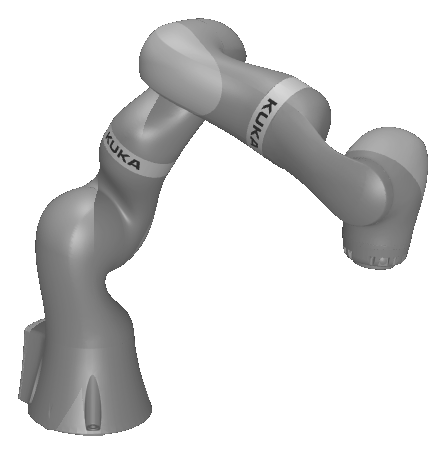
\includegraphics[width=4.0cm]{kuka_arm.png}};
\node[font=\footnotesize,align=center,text width=4.3cm] at (1.2,-1.0){KUKA iiwa14 (7 axes)\\meshes / masses / inertias\\from MuJoCo Menagerie};
% highlight joint i (fractional position over the image)
\coordinate (jhiX) at ($(kuka.south west)!0.34!(kuka.south east)$);
\coordinate (jhiY) at ($(kuka.south west)!0.62!(kuka.north west)$);
\coordinate (jhi) at (jhiX |- jhiY);
\node[draw=black,circle,line width=1.3pt,inner sep=3.5pt] at (jhi){};
\node[font=\footnotesize,left=2pt of jhi]{joint $i$};
% ===== zoom / exploded callout =====
\coordinate (zNW) at (3.5,1.22);\coordinate (zSE) at (9.7,-1.22);\coordinate (zSW) at (3.5,-1.22);
\draw[densely dashed,line width=0.6pt,rounded corners=4pt] (zNW) rectangle (zSE);
\draw[densely dashed,line width=0.6pt] (jhi) -- (zNW);
\draw[densely dashed,line width=0.6pt] (jhi) -- (zSW);
\node[font=\footnotesize\itshape] at (2.9,1.0) {exploded view};
% ===== (B) exploded flexible joint =====
\begin{scope}[shift={(7.4,0)}]
  \node[mass,fill=black!20,minimum width=1.5cm,minimum height=1.7cm] (motor) at (-3,0) {};
  \node[lbl] at (motor){\bfseries Motor\\(rotor)\\$J_m,\ \theta_m$};
  \draw[->,line width=1pt] (-5.5,0) -- (motor.west);
  \node[note,align=center] at (-4.75,0.42){actuator\\torque $\tau_m$};
  \node[mass,fill=black!5,minimum width=1.6cm,minimum height=1.9cm] (link) at (1.4,0) {};
  \node[lbl] at (link){\bfseries Link\\$J_\ell,\ \theta_\ell$};
  \draw[->,line width=1pt] (link.east) -- ++(1.15,0) node[right=1pt,font=\footnotesize]{next link};
  \draw[->,line width=0.9pt] (2.05,-0.95) -- ++(0,-0.85) node[below]{$g$};
  \draw[->,line width=0.9pt] (0.75,-1.8) -- (0.75,-0.95) node[pos=0,below]{$\tau_d$};
  \draw[decorate,decoration={coil,aspect=0.6,segment length=4.2pt,amplitude=5pt},line width=0.9pt]
        (motor.east|-0,0.55) -- (link.west|-0,0.55);
  \node[above] at (-0.8,0.74){$K$ (gear stiffness)};
  \draw[line width=0.9pt] (motor.east|-0,-0.55) -- ++(0.7,0);
  \draw[line width=0.9pt] (-1.45,-0.85) rectangle (-1.0,-0.25);
  \draw[line width=1.1pt] (-1.225,-0.8) -- (-1.225,-0.3);
  \draw[line width=0.9pt] (-1.225,-0.55) -- (link.west|-0,-0.55);
  \node[below] at (-0.8,-0.74){$d$ (damping)};
  \draw[dim] (motor.east|-0,1.52) -- (link.west|-0,1.52);
  \node[above,note] at (-0.8,1.57){$\Delta=\theta_m-\theta_\ell$ = transmission error};
  \node[enc,minimum width=1.3cm,minimum height=0.5cm] (encm) at (-3,-2.05) {$\theta_m$};
  \draw[->,line width=0.7pt] (motor.south) -- (encm.north);
  \node[note,below=1pt of encm,text width=3.2cm]{\textbf{Motor-side encoder}\\(what the controller assumes)};
  \node[enc,minimum width=1.5cm,minimum height=0.5cm] (encl) at (1.4,2.6) {$\theta_\ell=\theta_m+\Delta$};
  \draw[->,line width=0.7pt] (link.north) -- (encl.south);
  \node[note,above=1pt of encl,text width=4.9cm,align=center]
    {\textbf{Joint-side / output encoder} $\to$ \textbf{ILC}\\(reads the true link angle; true TCP is used for evaluation only)};
\end{scope}
\node[font=\footnotesize,align=left,text width=7.1cm,anchor=north west] at (6.5,-2.55)
  {$\tau_d$ (link disturbances, unknown to the controller) $=$ gear transmission error $K\varepsilon(\theta)$ $+$ Stribeck friction $+$ backlash $+$ thermal drift $K\,k_T\,T(t)$};
\end{tikzpicture}
\end{document}
